\section{Diffusion MRI Processing}
Synopsis (<100 words): Tractography based on diffusion-weighted MRI provides non-invasive in vivo estimates of trajectories of long-range brain connections. These estimates are important in research that measures individual differences in brain connections and in clinical use-cases. But the computational demands of tractography present a barrier to progress. Here, we present a GPU-based tractography implementation that accelerates tractography algorithms implemented as part of the Diffusion Imaging in Python (DIPY) project. This implementation speeds up tractography by at least a factor of ~200X, providing tractographies that closely match CPU-based solutions. These speedups enable applications of tractography in clinical data, and in very large datasets.

Summary (<250 characters): GPU-accelerated tractography algorithms that leverage the methods implemented in the DIPY open-source software project accelerate tractography by at least 200-fold, enabling applications to clinical data, as well as very large datasets. 

\section{DESIGNER}

\section{GPU-accelerated Diffusion MRI Tractography in DIPY}

\subsection{Methods}
DIPY (Diffusion Imaging in Python; \url{https://dipy.org}) is an open-source software library that implements many methods in computational neuroanatomy \cite{garyfallidis_dipy_2014}. Relying on the DIPY implementation of residual bootstrap tractography \cite{berman_probabilistic_2008}, we implemented a multi-GPU parallelizable version constructed on NVIDIA’s CUDA application programming interface (API).  The API of the GPU version is compatible with the one implemented in DIPY, enabling direct comparisons and interoperability. A docker container of the software makes the installation and use of the software straightforward. The software is available at \url{https://github.com/dipy/GPUStreamlines}. Experiments to profile the performance of the algorithm were conducted using an AWS $p3.16\textrm{xlarge}$ instance with 8 NVIDIA Tesla V100 Graphical Processing Units and 488 GB RAM. For comparison, CPU code was run on an AWS $x1e.4\textrm{xlarge}$ with 488 GB RAM. We used two datasets, the first is a HARDI acquisition with 2x2x2 mm3 isotropic voxels, 150 b=1,000 s/mm2 volumes and 10 b0 volumes previously described in \cite{rokem_evaluating_2015}. The other dataset was a Super-Resolution Hybrid Diffusion Imaging  (HYDI) dataset \cite{Garyfallidis2019}, with an effective resolution of 0.625 mm3 isotropic voxels, b=500, 800, 1600, 2600 s/mm2, in 134 diffusion directions, and 8 b0 volumes, also previously described in \cite{elsaid_super-resolution_2019}. In both cases, 27 seeds were placed in each voxel in the white matter to initialize tracking.

\subsection{Results} 
In the HARDI dataset, with the seeding approach used
here, approximately 2.1M streamlines were generated. Using the CPU-based
residual bootstrap tracking algorithm took approximately 13 hours. The
GPU-accelerated implementation provides approximately 200-fold speedup
with a single GPU, and up to 671-fold speedup with 8 GPUs run in
parallel (Figure \ref{fig:gpu_speedup}). In the HYDI dataset, the seeding approach used generated 150M streamlines (497GB). Tracking in this case with 8 GPU
completed in just under 2 hours. A subset of the HYDI streamlines are
shown in Figure \ref{fig:gpu_streamlines}.

\begin{figure}[htbp]
    \centering
    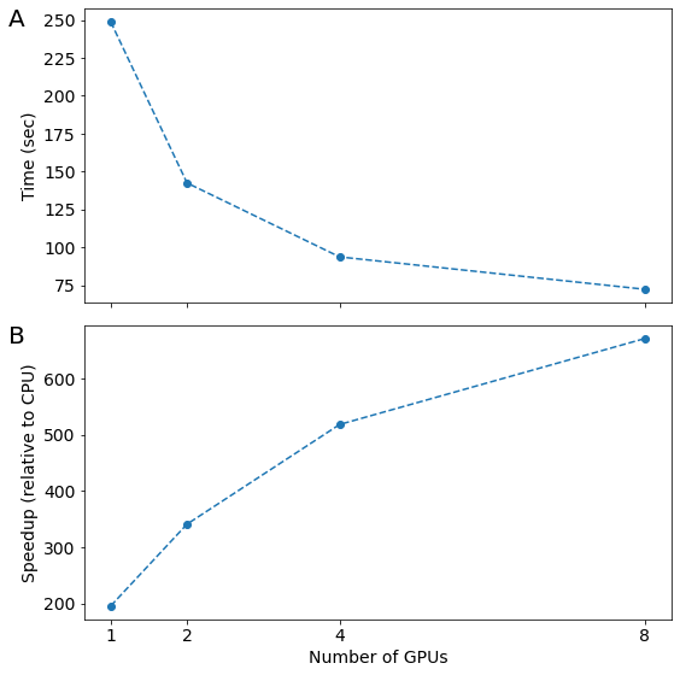
\includegraphics[width=\textwidth]{../figures/chapter2/speedup.png}
    \caption{For the same task (HARDI data, 27 seeds per WM voxel) tractography duration decreases with the number of GPUs available. Speedup relative to CPU ranges from approximately 200-fold, with one GPU to almost 700-fold with 8 GPUs.}
    \label{fig:gpu_speedup}
\end{figure}

\begin{figure}[htbp]
	\centering
	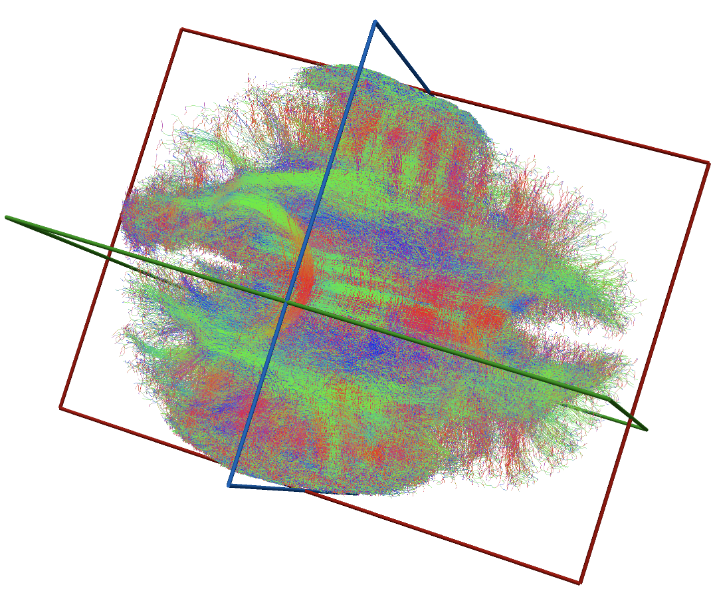
\includegraphics[width=\textwidth]{../figures/chapter2/streamlines.png}
	\caption{GPU-accelerated tractography of high-resolution data, acquired at 0.625 mm3  effective resolution. This is a small subset sampled randomly for visualization purposes: approximately 8M streamlines of the 150M streamlines tracked.}
	\label{fig:gpu_streamlines}
\end{figure}

\subsection{Discussion and Conclusion} 
A GPU-based implementation of residual bootstrap tractography provides orders of magnitude speedup, relative to the CPU-based version, while providing solutions that match CPU-based solutions very closely. This was demonstrated in standard and high-resolution measurements. Thus, this GPU-based implementation allows
researchers to both (1) save time and money solving existing problem
sizes and (2) solve new problems that are computationally intractable on
CPU-only resources. Open-source software is provided, as well as a
docker container that encapsulates the software, together with all of
its dependencies available at
\url{docker.pkg.github.com/dipy/gpustreamlines/gpustreamlines}.
